\subsection{Organisation du programme}
Le projet contient :
\begin{itemize}
\item un \verb+README+, avec le mode d'emploi pour installer les dépendances ;
\item un répertoire base / avec plusieurs librairies externes (sous
licences compatibles GPLv2) ;
\item un fichier de configuration ;
\item \verb+queue.h/cc+, \verb+packet.h/cc+ et \verb+conntrack.h/cc+ qui réalisent l'interception des paquets envoyés à \verb+NFQUEUE+ (\verb+queue.cc+), leur
interprétation (\verb+packet.cc+), et leur mise en relation avec un conntrack
(\verb+conntrack.cc+) ;
\item \verb+classifier.h/cc+ qui sert à classer les paquets ;
\item un fichier de base permettant le lancement des thread, un autre parsant le fichier de configuration et initialisant le classifier.
\end{itemize}

\subsection{Fonctionnement du logiciel}
Nous avons utilisé la \verb+libnetfilter_conntrack+ pour
récupérer les entrées conntrack existantes du noyau, et afin de maintenir une table locale dans le but d'éviter de se poser la question de la suppression des vieilles entrées.

\begin{figure}[h]
\centering
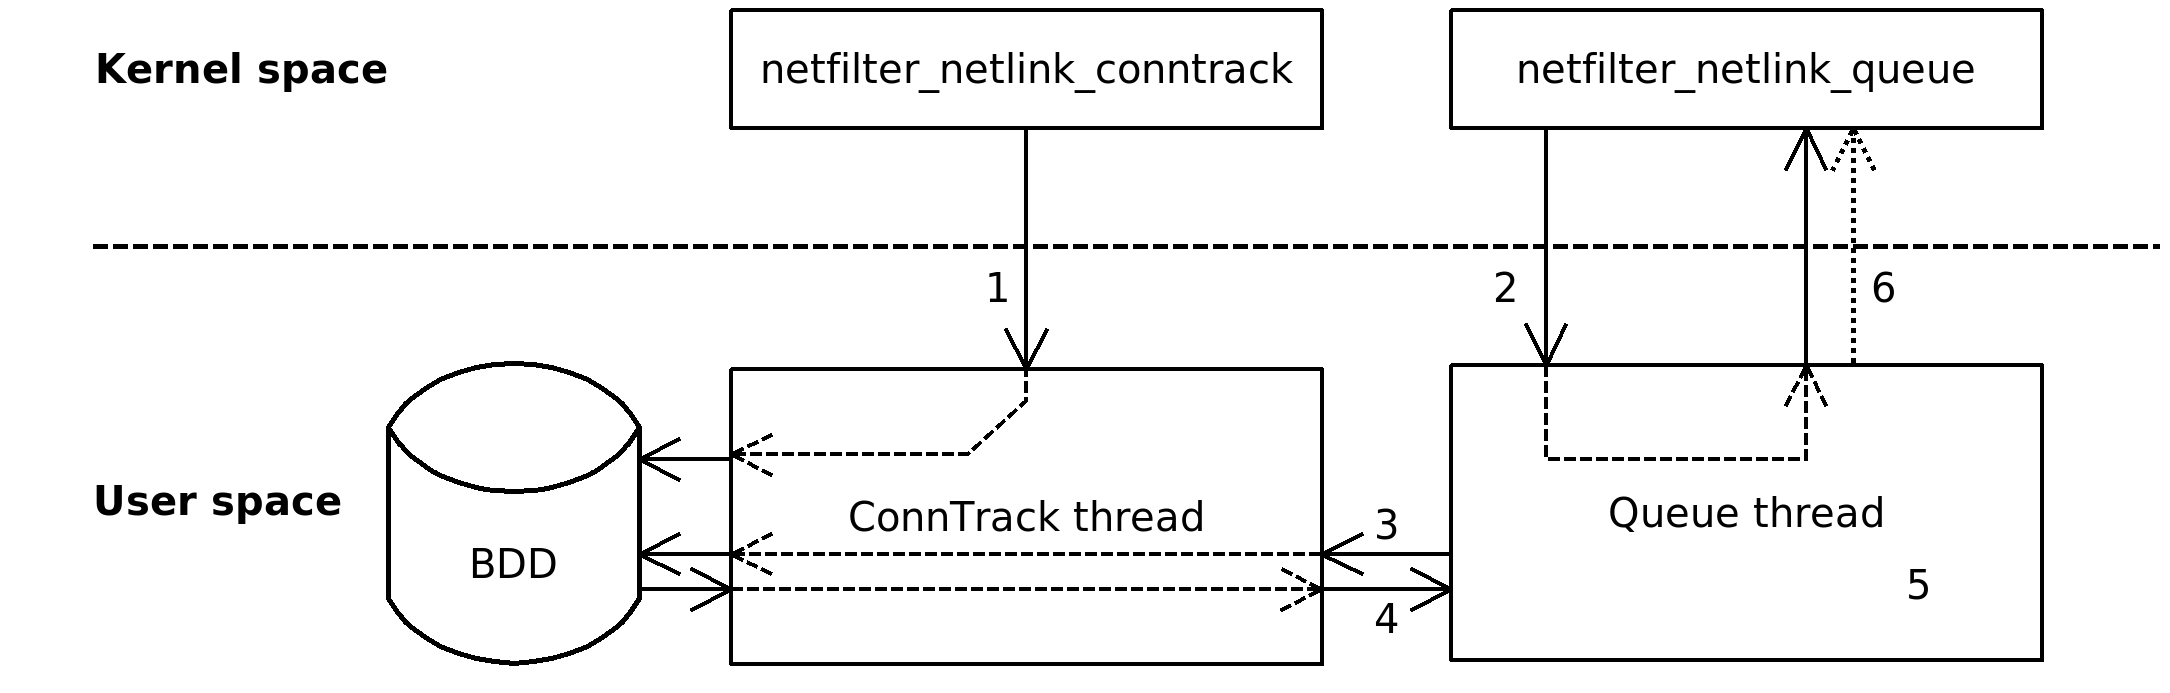
\includegraphics[width=\textwidth]{schema2.png}\\
\title{Fonctionnement du module}
\end{figure}

\begin{footnotesize}
\noindent Légende du schéma :

\begin{enumerate}
\item Maintien d'une copie locale de la base conntrack du noyau, grâce aux \og events \fg{} de la \verb+libnetfilter_conntrack+.
\item Récupération des paquets envoyés sur \verb+NFQUEUE+ via la \verb+libnetfilter_queue+.
\item Récupération, pour chaque paquet, des informations de conntrack existantes.
\item Retour des informations de conntrack pour le paquet, en particulier le contenu des paquets précédents, pour permettre la classification.
\item Classification basée exclusivement sur le contenu de la connexion.
\item Réinjection du paquet et d'une \og mark \fg{} de classification dans la chaîne de filtrage netfilter du noyau.
\end{enumerate}
\end{footnotesize}

Il y a deux threads ; le premier (cf. \verb+ConnTrack::Run()+) écoute sur un
\verb+netfilter_netlink+, reçoit les mises à jour de la table conntrack du noyau, et
maintient une copie locale.\\

Le deuxième (cf. \verb+Queue::Run()+) intercepte les paquets arrivant sur une
\verb+NFQUEUE+ (via \verb+iptables+), les parse, détermine l'entrée conntrack
correspondante (en demandant à une table partagée avec l'autre
thread), récupère l'object \og Connection \fg{} correspondant, met à jour les
deux buffers, puis appelle la méthode \verb+update+ du classifier ; enfin il
accepte le paquet, en le marquant avec la mark déterminée par le
classifier (ou une marque par défaut si pas de classifier).\\

Le classifier regarde les buffers d'une connection à chaque fois que les buffers d'une connection à chaque fois qu'ils sont mis à jour. Il prend ensuite une décision (NoMatch, NoMatchYet ou une vraie décision) ; le classifier retourne aussi un \og buffer hint \fg{} au conntrack : c'est à dire qu'il indique quelle
partie du buffer lui est encore utile, pour que le conntrack puisse
purger la partie inutile du buffer.\\

Le cheminement des paquets, avec une extension en userspace, sera le suivant :\\
filtrage \verb+iptables+ et envoi vers la target \verb+NFQUEUE+\\
\verb+->+ récupération par le démon userspace, classification, et apposition d'une mark\\
\verb+->+ retour dans le noyau vers la chaîne \verb+iptables+ suivante (\verb+POSTROUTING+ par exemple si le paquet a été intercepté dans la chaine \verb+FORWARD+)\\
\verb+->+ éventuel refiltrage (en utilisant \verb+-m mark+ pour filtrer sur la mark).

\subsection{Quelques remarques et comparaisons avec l7-filter}
Le \verb+l7-filter+ userspace utilisait un conntrack fait main alors que nous utilisons le conntrack du noyau. Cela devrait être plus efficace parce que cela permettra dans quasiment tous les cas de savoir qui est le client qui est le serveur à l'exception du cas où un paquet arrive sur \og queue \fg{} avant que l'information de conntrack n'arrive dans l'autre thread.\\

Une fois qu'un paquet a été envoyé à \verb+NFQUEUE+, il ne peut pas passer
tant qu'un démon userspace ne l'a pas accepté ; donc si notre application est
DOSsée et plante, le pirate aura perdu puisque plus rien ne passera.\\

Il y a une limite sur la taille du buffer (buffer-size limit). Cela fait en sorte que si le
buffer d'une connection dépasse une certaine taille, la connection
passe en NoMatch (si le BufferHint est bien respecté par le
classifier, cela n'arrivera pas dans les cas qui nous intéressent).\\

Par ailleurs, notre programme supporte l'IPv6 alors que \verb+l7-filter+ ne le supportait pas.
